% -------------------------------------
% |   Made with Hate by Captain Joni  | 
% -------------------------------------



\documentclass{include/berichtclass}
\usepackage{wrapfig}
\usepackage[numbers]{natbib}




\SelectLanguage{ngerman}


%--------------------
%|   Definitionen   |
%--------------------


\newcommand{\abbildung}[4]{
	\begin{figure}[ht]
		\centering
  		\includegraphics[width=#1\textwidth]{#2}
		\caption{#3}
		\label{#4}
	\end{figure}
}



%% -----------------------------------------------
%% |    Einstellungen zu jedem Versuch           |
%% -----------------------------------------------


\newcommand{\versuch}{Versuch 22 - Bestimmung der Elementarladung nach Milikan}
\newcommand{\datum}{01.10.2025}


%  ---------------------
% | Einmal Einstellungen |
%  ----------------------
\newcommand{\name}{Paul Saß}
\newcommand{\gruppe}{9}
\newcommand{\Kurs}{Vormittags}
\newcommand{\tutor}{Louis Laschinger}






%% ------------------------------
%% |    Versuchsausarbeitung    |
%% ------------------------------
\begin{document}
    % Titlepage
 
    \FrontMatter
    % Die Titelseite

\begin{titlepage}

\vspace{20mm}
\begin{center}
\scalebox{1.6}{
    \textbf{\Large Versuch 22 - Bestimmung der}
    
    } \par
\scalebox{1.6}{
    \textbf{\Large Elementarladung nach Milikan} 
    } \par 
    
    \vspace{20mm}
    \scalebox{1.3}{
    \textbf{\Large PAP 1}}
    \par
    \vspace{10mm}
    \scalebox{1.2}{
    \datum} \par
    \vspace{100mm}


    

\vspace{50mm}
    Teilnehmender Student: \textbf{\name} \par
    Gruppe: \gruppe \par
    Kurs: \Kurs \par
    Tutor/in : \tutor \par
\end{center}
\end{titlepage}
    \begingroup \let\clearpage\relax

    \pagestyle{plain}


    
    \newpage
    \tableofcontents
    \endgroup
    

    % Contents
    \MainMatter
    \begingroup
    \let\clearpage\relax





% Die Texte werden in den einzelnen Dateien eingefügt.
    \chapter{Einleitung}
    \section{Motivation}



\section{Messverfahren}
Für das Experiment wird ein Spektrophotometer, welches aus einer Lampe, einer Linse, einem Küvettenhalter und einem
Gitterspektrometer besteht. In dem Gitterspektrometer wird das Licht auf einen CCD Sensor gestreut und damit die
Intensität des Lichts gemessen.

\subsection{Messung des Absorptionsspektrums}
ZU Beginn wird die 6 cm Küvette mit fester Konzentration Kaliumpermanganat verwendet um mit dem Gitterspektrometer
die Wellenlängen der Absoptionsmaxima zu bestimmen. Zuvor wird das Spektrometer mit einer Dunkelmessung und 
einer Messung ohne Küvette kalibriert.

\subsection{Absorption in Abhängigkeit der Küvettenlänge}
Für diese Messung wurde die Menge des Absorbierten Lichts bei einer festen Wellenlänge und varrierter
Küvettenlänge gemessen. Dies wurde für jede Küvette fünf mal wiederholt.

\subsection{Absorption in Abhängigkeit der Konzentration}

Für diese Messung wurde bei konstanter Wellenlänge und variabler Konzentration gemessen. Dabei wurden jeweils fünf Messungen
durchgefüht und danach die Kaliumpermanganatkonzentration erhöht.



\section{Grundlagen aus der Physik}

\subsection{Küvette}
Bei dem Durchlaufen des Lichts durch die Küvette wird das Licht leicht gebeugt, da die Küvette nicht Fehlerfrei ist.
Aus dem Messen der Durchmesser der Lichtkegel mit Küvellte $D_{mK}$ und ohne Küvette $D_{oK}$ lässt sich die Ablenkung berechnen und eliminieren:
\begin{equation}
    I_{korr} = I \cdot \frac{D_{mK}^2}{D_{oK}^2}
    \label{eq:Ikorr}
\end{equation}

\subsection{Stoffmengee und Konzentration}
Ein mol enpricht $6,022 \cdot 10^{23}$ Teilchen. Die Konzentration beschreibt die Anzahl von
Teilchen pro Volumeen. Dabei ist die Einheit $\tfrac{mol}{l}$.
Um bei einem hinzugefügten Volumen $V_j$ der Kaliumpermanganatlösung die Konzentration
zu bestimmen wird mithilfe des Ausgabsvolumen $V_0$, den einzel Volumina $V_j$ und der 
Konzentration $\tilde{c}$ des konzentrierten Kaliumpermangantas folgende Formal angewendet:
\begin{equation}
    c = \tilde{c} \frac{\sum_{i=1}^n V_i}{V_0 + \sum_{i=1}^n V_i}
    \label{eq:Konzentration}
\end{equation}

\subsection{Das Lambertsche Absorptionsgesetz}
Das Lambertsche Absorptionsgesetz vermittelt das fundamentale Verständniss der Lichtabsorption
in Lösungen. Nach diesem nimmt die Intensität exponentiell über den Verlauf durch das Medium ab.
Daraus folgt:

\begin{equation}
    I = I_0 \cdot e^{-kl}
\end{equation}
Dabei sind:
\begin{itemize}
    \item $I_0$ die Ausgangsintensität
    \item $k$ den Absoptionskoeffizienten
    \item $l$ die durchschrittene Länge in der Lösung
\end{itemize}


\subsection{Das Gesetz von Beer}
In einer verdünnten Lösung ist der Absorptionkoeffizient $k'$ proportional zur Konzentration $c$.
Diese unterscheiden sich in einem Faktor $\epsilon$ dem molaren Extinktionskoeffizienten. Diese
ist eine Stoffkonstante, welche die Absorption des Lichts einer bestimmten Wellenlänge angibt.

\begin{equation}
    k' = \epsilon \cdot c
    \label{eq:dekAbsorp}
\end{equation}

Aus der Verknüpfung dieser Beiden Gesetze folgt:
\begin{equation}
    I = I_0 \cdot 10^{-\epsilon k l}
\end{equation}
Bei der umrechnung in die Zehner-Basis wird $k' = \log(e) k$ verwendet.

    \newpage
    \chapter{Durchführung}
    \section{Versuchsaufbau}
\begin{figure}[h!]
    \centering
    \includegraphics[page=1, width=1\textwidth,]{IMG_CCB29F6F352C-1.jpeg}
    \caption{Aufbau}
\end{figure}
\newpage
\section{Messprotokoll}
\begin{figure}[h!]
    \centering
    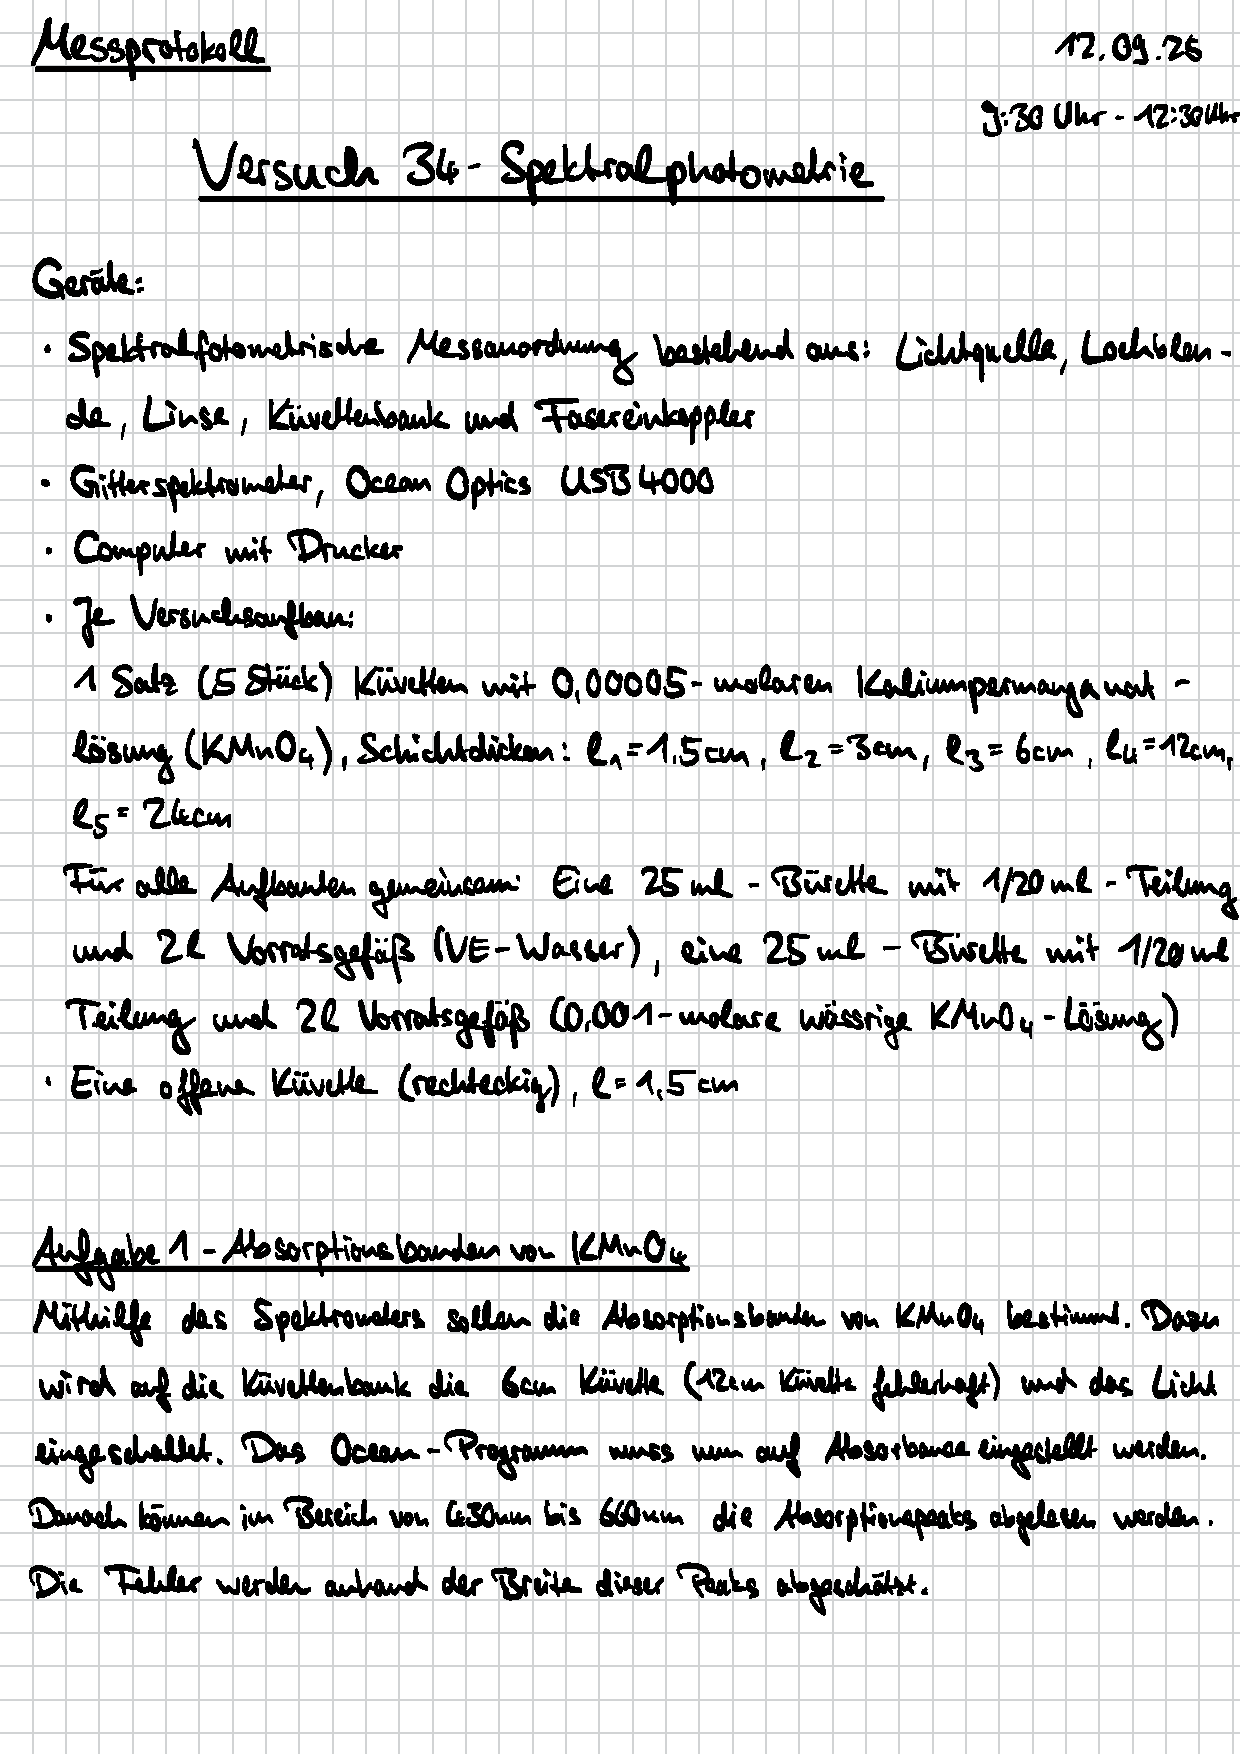
\includegraphics[page=1, width=1\textwidth,]{Versuch34.pdf}
    \caption{Messprotokoll Versuch 34 Seite 1}
\end{figure}
\newpage
\begin{figure}[h!]
    \centering
    \includegraphics[page=2, width=1\textwidth,]{Versuch34.pdf}
    \caption{Messprotokoll Versuch 34 Seite 2}
\end{figure}
\newpage
\begin{figure}[h!]
    \centering
    \includegraphics[page=3, width=1\textwidth,]{Versuch34.pdf}
    \caption{Messprotokoll Versuch 34  Seite 3}
\end{figure}
\newpage
\begin{figure}[h!]
    \centering
    \includegraphics[page=4, width=0.95\textwidth,]{Versuch34.pdf}
    \caption{Messprotokoll Versuch 34 Seite 4}
\end{figure}
\newpage
\begin{figure}[h!]
    \centering
    \includegraphics[page=5, width=1\textwidth,]{Versuch34.pdf}
    \caption{Messprotokoll Versuch 34  Seite 5}
\end{figure}
\newpage
    \newpage
    \chapter{Auswertung}
    \section{Aufgabe I}

\begin{table}[h!]
    \centering
    \begin{tabular}{c r r}
        \toprule
        Messung & Gemessene Zeit [s] & Umlaufzeit $T_0$ [s] \\
        \midrule
        1 & $36,32 \pm 0,3$ & $ 1,816 \pm 0,015$ \\
        2 & $36,34 \pm 0,3$ & $ 1,817 \pm 0,015$ \\
        3 & $36,31 \pm 0,3$ & $ 1,816 \pm 0,015$ \\
        \bottomrule
        \multicolumn{3}{c}{$\overline{T_0} = 1,816 \pm 0,015$}
    \end{tabular}
\end{table}
Fehler:

\begin{equation}
    \Delta \overline{T_0} = \sqrt{\sigma^2 + (\Delta T_0)^2}
\end{equation}

Wobei $\Delta T_0$ die Abweichung einer Umlaufzeit ist, also die Reaktionszeit heruntergerechnet auf einen Umlauf und $\sigma$ die
mittlere Abweichung des Mittelwerts ist.
    \newpage
    \chapter{Zusamenfassung und Diskussion}
    
\section{Wasserwert}

Der berechnete Wasserwert liegt bei $\boxed{W= ( 95 \pm  17)\ \tfrac{\text{J}}{\text{K}}}$.
Verglichen mit dem angegebenen Wert von $70\ \tfrac{\text{J}}{\text{K}}$ ergibt sicht eine Abweichung
von $1,5 \sigma$. Der gemessene Wert liegt noch gut im $3\sigma$ Bereich. Deshalb ist der Wert mit
dem angegebenen vereinbar und kann als genau anerkannt werden.
Die größte Fehlerquelle liegt höchstwarscheinlich in der genauen bestimmung der Wassertemperatur vo der Messung.
Durch den Einschüttvorgang konnte das Wasser Wärme an die Umgebungsluft abgeben wodurch es kälter als erwartet im Kalorimeter angelangt ist.
Daraus resultierte eine kühlere Gleichgewichtstemperatur und dementsprechend ein höherer Wasserwert. Allerdings schwangt die Wärmeisolierung von Gerät zu Gerät weshalb der Vergleich nicht für alle Geräte Sinnvoll ist.

\section{Spezifische Wärme Kalorimeter}
Die Ergebnisse von Aluminium mit $\boxed{c_m = 0,84 \pm 0,03\ \tfrac{\text{J}}{\text{gK}}}$ und Blei $\boxed{c_m = 0,13\pm0,01\ \tfrac{\text{J}}{\text{gK}}}$
sind mit Abweichungen von $2\sigma$ und $0,1\sigma$ als Erfolgreich zu bewerten. Bei der Blei Messung
hätten die Fahlerabschätzungen verringert werden können um das Ergebnis genauer eingrenzen zu können.\\
Auffällig ist hingegen das Ergebnis von Graphit  $\boxed{c_m = 0,77\pm0,02\ \tfrac{\text{J}}{\text{gK}}}$. Dieses erzielt eine Abweichung von $3\sigma$.
Dieser Bereich gilt zwar als akzeptabel jedoch muss das Ergebnis kritisch betrachtet werden.
Einen Fehler könnte der Wasserwert sein, jedoch müsste dieser Fehler auch auf die anderen Werte zutreffen.
Es muss auf einen systematischen Fehler geschlossen werden, bei welchem kleine Fehler in der Versuchdurchführung passiert sind.\\
Besonders auffällig ist ebenfalls die hohe Abweichung von $70\sigma$ bei Graphit von der Dulong-Petit Methode.
Das Problem bei der Dulong Petit methode ist, dass sie bei leichten Elementen wie Kohlenstoff versagt. Das kommt, da die
Schwingungen sehr Hochfrequent sind und deshalb die Energiezustände nicht vollständig angeregt sondern quantisiert sind.


\section{Spezifische Wärme Stickstoff}
Zu erwarten ist, dass die gemessenen Kapazitäten etwas zu hoch sind.
Der ausschlaggebenste Grund dafür wäre eine Verdunstung des Stickstoffs aufgrund des Kontaks zur Luft mit Zimmertemperatur.
Dadurch steigt die Massendifferenz und demnach auch die berechnete Wärmekapazität. Ebenfalls kann Stickstoff beim Sieden aus dem Dewargefäß heraussprudeln,
was ebenfalls zu einem erhöhten Massenverlust führt.
Dieser Effekt ist auch bei dieser Messung zu erkennen:
\begin{align}
    \boxed{c_C = 0,5098 \pm 0,0023 \ \tfrac{\text{J}}{\text{gK}} \quad c_{Al} = 0,759 \pm 0,003 \ \tfrac{\text{J}}{\text{gK}} \quad C_{Pb} = 0,1298 \pm 0,0006 \ \tfrac{\text{J}}{\text{gK}}}
\end{align}

Das diese Werte zu klein sind erkennt man aber nicht direkt, da keine Literaturwerte als Referenz angegeben sind.
Daher müssen dafür die Debye-Temperaturen betrachtet werden.

\section{Debye-Temperaturen}
Die abgelesenen Debye Temperaturen sind:
\begin{align}
    \boxed{\Theta_{C} = 80 \pm 18 \ \text{K} \quad \Theta_{Al} = 210 \pm 10 \ \text{K} \quad \Theta_{Pb} = 630 \pm 30 \ \text{K}}
\end{align}

Die Debye-Temperaturen sind direkt abhängig von dem Verhältnis der Wärmekapazitäten bei den beiden Messtemperaturen.
Die Debye Temperatur von Blei kann mit einer Abweichung von $0,8 \ \sigma$ als genau betrachtet werden. Da dort ebenfalls der Wert der spezifischen Wärme
als erfolgreich gemessen betrachtet wird, gilt hier auch für den Messwert bei Stickstoff, dass dieser erfolgreich gemessen wurde.
Dies kann angenommen werden, da die Messtemperatur bei Stickstoff direkt abhänig von der Debye-Temperatur und der Wärmekapazität im Kalorimeter abhängt.\\

Auffällig sind die Debye-Temperaturen von Aluminium und Graphit. Die Abweichungen betragen hier $22 \ \sigma$ und $50 \sigma$.
Beim Aluminium ist auf einen Messfehler in der Stickstoffmessung zu schließen welcher auf die oben genannten systematischen Fehlerquellen zurückzuführen sein muss, da auch hier der
Messwert aus dem Kalorimeter genau ist.\\
Bei Graphit ist die Ermittlung der Fehlerquelle etwas komplexer wobei natürlich die gleichen systematischen Fehler wie für das Aluminium gelten.
Jedoch gilt der Literaturwert zum Vergleich für Diamant, da Graphit keine einheitliche Debye-Temperatur festgesetzt ist.
Aufgrund dessen ist als Fehlerquelle hier auch der Literaturwert zu berücksichtigen.
Allerdings ist die Abweichung von $50 \ \sigma$ zu groß um es bei einer simplen Abweichung des Literaturwerts zu belassen.
Die Messung muss hier als Fehlerhaft betrachtet werden. Bei Graphit wird der größte Fehler in dem unkontrollierten Verdunsten des Stickstoffs liegen.
Da die Graphit-Ptobe am größten war, ist nicht auszuschließen, dass flüssiger Stickstoff durch das Sieden aus de mGefäß gelangt ist.

\section{Zusammenfassung}

Zusammenfassend lässt sich sagen, dass der Versuch im allgemeinen erfolgreich war.
Die Werte lagen meist in dem 3 $\sigma$ der Literaturwerte. Daher können diese als Bestätigung der Literaturwerte angesehen werden.
Jedoch sollte die Messung der Werde des Grphits widerholt werden, da dort der Wert der Debye-Temperatur sehr starrk von dem Rreferenzwert abweicht.\\

Zu verbessern an der Vrsuchsdurchführung wäre das verwenden größerer Dewargefäße um einerseits die Isolation gegen
die Umluft zu vebessern und andererseits das Risiko eines Massenverlustes durch das Überschwappen des siedenden Stickstoffs zu minimierren.\\
Dazu kommt, dass das Thermometer teilweise sehr lang gebraucht hat um eine konstante Temperratur anzuzeigen. Dies könnte besonders in der Messung des Wasserwerts Fehlerr hinterlassen haben.
Demenstprechend wäre ein Thermometer besser geeignet, dass sich schneller einstellt.


    \endgroup

    \newpage
    \begingroup \let\clearpage\relax  


    \endgroup

\end{document}

% ---------------------------
% |   Made by Captain Joni  | 
% ---------------------------
